\documentclass[journal]{IEEEtran}
\usepackage{cite}
\usepackage[dvips]{graphicx}
\usepackage{hyperref}
\usepackage{wrapfig}
\newcommand{\extraSpace}{\vspace{30pt}}

\begin{document}
\title{Optical phase characterization of photonic integrated devices}
\author{J.~Matres,~G.~C.~Ballesteros,~S.~Mas,~A.~Brimont,~P.~Sanchis,~J.~Marti~and~C.~J.~Oton}
\markboth{IEEE JOURNAL OF SELECTED TOPICS IN QUANTUM ELECTRONICS}{Shell \MakeLowercase{\textit{J. Matres et al.}}: Optical phase characterization of integrated photonic devices}
\maketitle

\begin{abstract}
We propose a relatively simple experimental setup, capable of accurately characterizing the optical phase response of an integrated photonic circuit.
The setup is based on a phase-noise reduction scheme using an external heterodyne Mach–Zehnder interferometer.
In particular, we characterize the phase response of different silicon photonic components: under- and over-coupled ring resonators, and a slow-light corrugated waveguide.
\end{abstract}

\section{Introduction}
\noindent In the last years, integrated optics has experimented a remarkable development thanks to technological advances but also because its recent trend towards standardization.
The main advantage of photonic integrated circuits is that one can build extremely complex systems with hundreds of components on a very small footprint and at a very low cost per device.
The phase response of an element is a key parameter that is required for the design of a system which includes it.
However, measuring the phase response is not straightforward, as under normal circumstances, phase noise complicates interferometric measurements using for example an external Mach-Zehnder interferometer (MZI).

\emph{Optical vector network analyzers} (OVNA) are commercial instruments sensitive to phase~\cite{Vanwiggeren2003, Gifford2005}.
They employ specific techniques to alleviate phase noise problems in their measurement, requiring complex synchronous receiving schemes with fringe monitoring and very fast laser tuning speeds (usually higher than 100~nm/s).
Fast laser sweeping reduces phase noise, as thermally-induced noise usually has a 1/f spectral dependence.


In this work, we present an alternative technique for measuring the phase response of a photonic component, using an ordinary laser with a tuning speed below 1~nm/s, without needing thermal control or isolation.
To achieve this, we cancel the phase noise employing a counter-propagating reference beam at fixed wavelength.
The concept of heterodyne measurement with two different wavelengths simultaneously is called superheterodyne detection~\cite{Dandliker1988}.
The fixed wavelength is used as a reference to cancel thermal phase fluctuations, while the tunable beam scans the desired spectrum.
In Ref.~\cite{Mas2012} we applied the same idea to characterize chromatic dispersion in waveguides with different geometries.
In this paper we show that the technique can be used as a general tool to characterize any photonic component.
In particular, we characterized a silicon microring resonator and a slow-light corrugated waveguide.
In the former, we distinguish under- from over-coupling conditions and extract the parameters of the ring.
In the latter, we plot the group index of the corrugation from a single segment of waveguide without the need of integrated MZIs and fringe spacing calculations.
The results show that the proposed technique provides an accurate measurement of the phase, being particularly useful for the characterization of slow-light photonic structures and other phase sensitive components.
Its main limitation is that it requires the compensation of the component delay with an external optical delay line.


\section{Experimental setup}
The experimental setup is a fiber-based MZI, where acousto-optic modulators (AOM) act as frequency shifters (Fig.~\ref{fig:dispersionSetup}).
Each branch applies a slightly different frequency shift (40~kHz in our experiment) and the lock-in amplifier measures the 40~kHz beating pattern (spectra are acquired in discrete tuning steps, therefore the beating frequency is not affected by the tuning speed).
The phase of these beatings with respect to the RF generators provides the phase of the system, but they are affected by thermal phase noise as high as several radians per second. 
This noise would make a phase characterization unfeasible using a laser with few nm/s tuning speed.
To cancel the phase noise, we introduce from the opposite end a reference counter-propagating beam at a fixed wavelength.
This signal produces another beating pattern used as a reference for the lock-in amplifier.
As thermal fluctuations equally affect both beams, they cancel out, measuring only the wavelength-dependent phase variations.


\begin{figure}[htb]
	\centering
	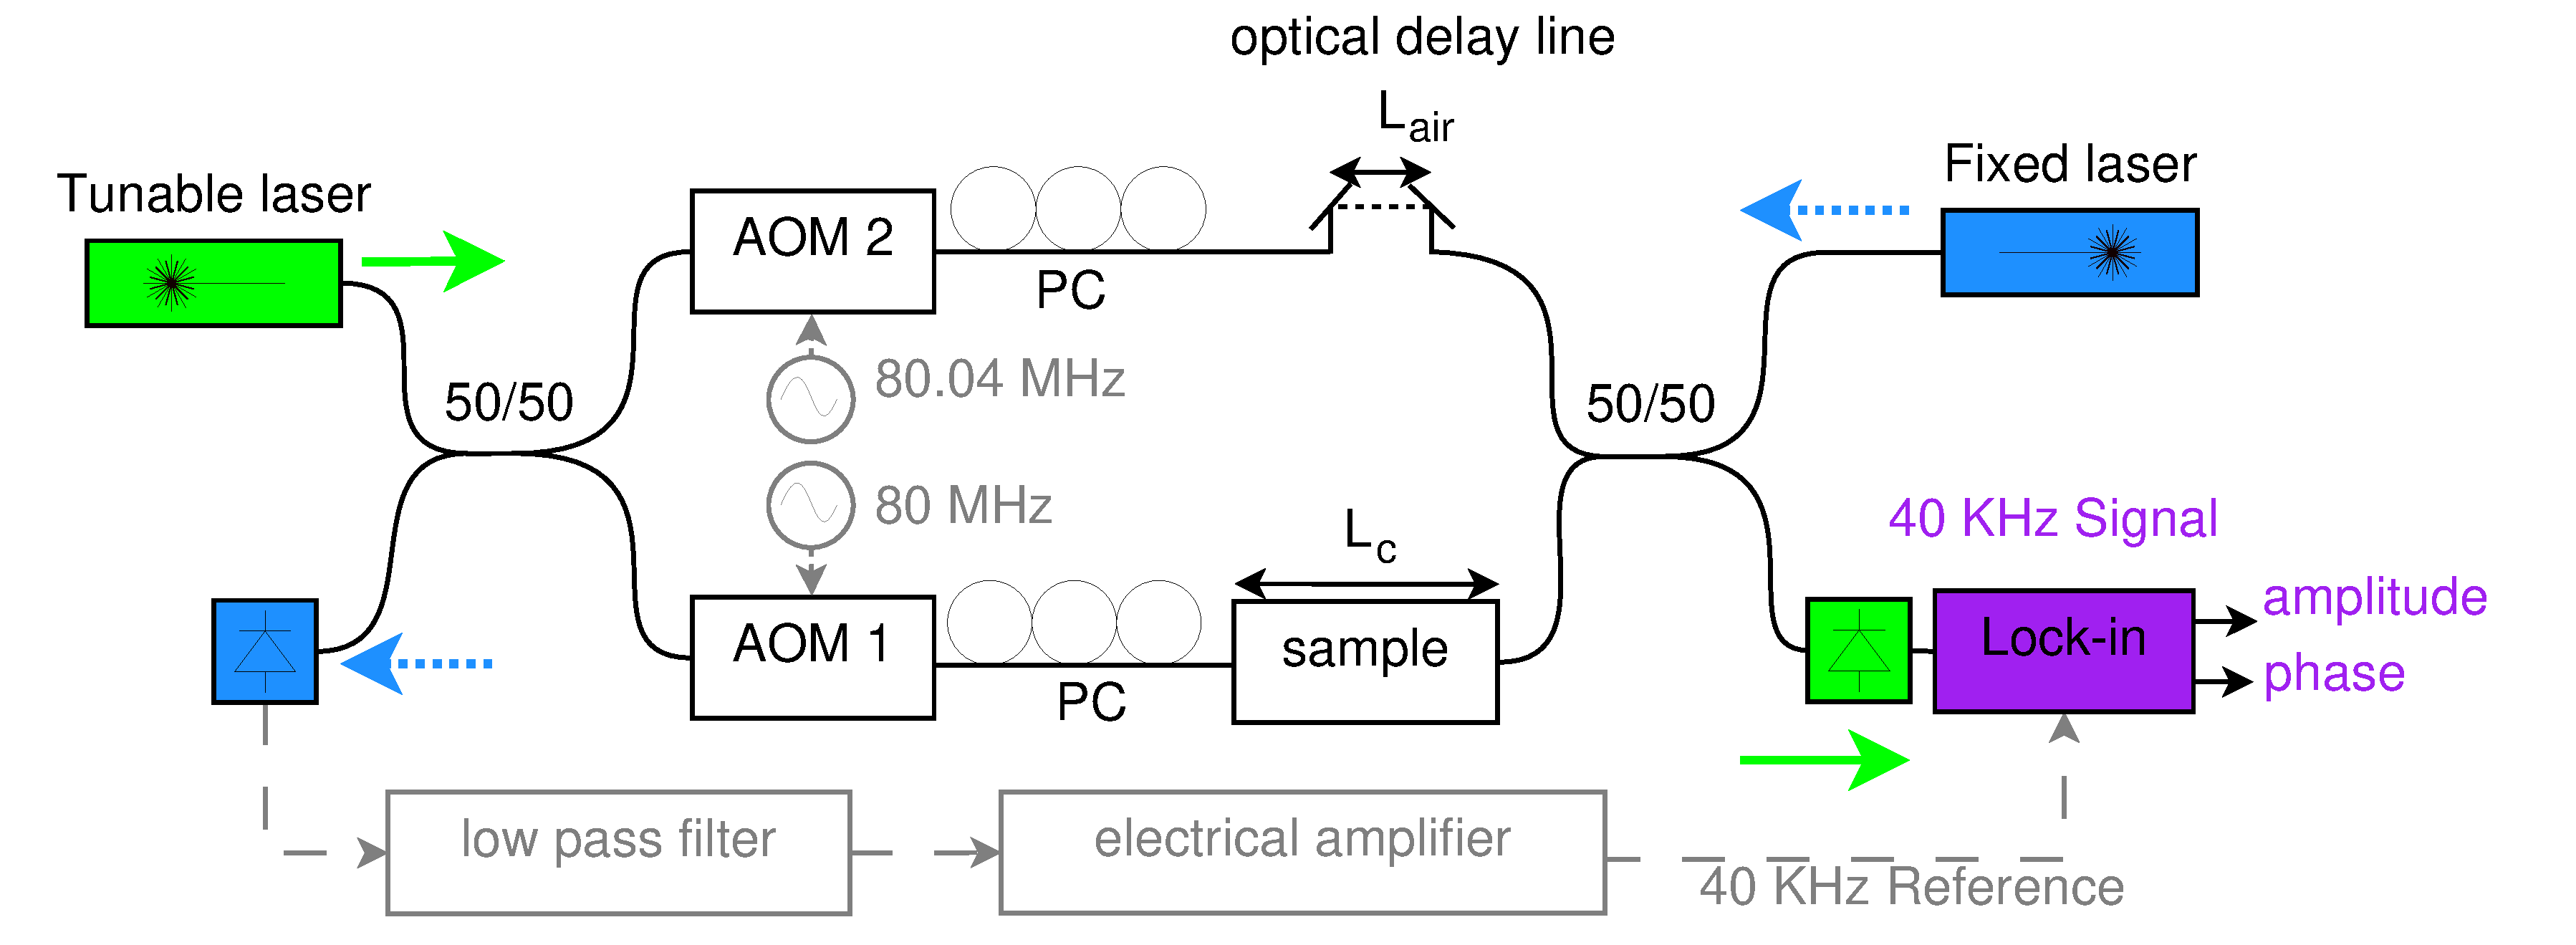
\includegraphics[width=3.5in]{dispersion6}
	\caption{Schematic of the experimental setup (the black lines represent standard single-mode fiber).
	The lock-in monitors the 40~KHz-beatings using a counter-propagating beam as a reference signal to compensate thermal fluctuations.
	AOM: acousto-optic modulator, PC: polarization controller. }
	\label{fig:dispersionSetup}
\end{figure}

To balance the interferometer for different device lengths there is an optical delay line in the branch without sample.
Before each sweep is launched, the MZI must be balanced in order to avoid too steep slopes in the $\omega$ phase dependence which could complicate the phase unwrapping.
In addition, it is convenient to set the wavelength of the counter-propagating reference beam, $\omega_0$, approximately in the middle of the sweep in order to minimize the phase noise.
If the building block to characterize is in series with other elements, (couplers, connecting waveguides, tapers, etc.), the measurement requires a reference sample with the same elements, but without the component under test (e.g. the corrugated waveguide). If the sample is entirely homogeneous, for example a straight waveguide, the reference measurement would be the trace with no sample.
The reference sweep provides the system response, which must be subtracted from the measurement with the component under test. 
Mathematically, the phase dependence obtained with the lock-in, after subtracting the system response, becomes:


\begin{equation}
  \phi(\omega)= \beta_c L_c - \beta_{air} \Delta L_{air} =\phi_{c}(\omega)-\frac{\omega\Delta L_{air}}{c}
  \label{eq:response}
\end{equation}

where $\phi$ is the measured phase, $\phi_{c}$ the phase introduced by the component under test, the extra length introduced in the optical delay line to balance the MZI with respect to the reference measurement is $\Delta L_{air}$, $\beta_c$ and $\beta_{air}$ are the propagation constants of the component and of air respectively, and $c$ the speed of light in vacuum.
In Ref.~\cite{Mas2012} we showed that if the component under test has a length $L_{c}$, then the group index of the component is:

\begin{equation}
  n_{g} = \frac{\Delta L_{air}}{L_{c}}
  \label{eq:group_index_pathBalancing}
\end{equation}

Minimizing the phase versus wavelength slope balances the MZI.
A slope equal to zero at a certain wavelength corresponds to perfect balancing, so one can extract the group index of the component under test.
Finally, we extract its wavelength dependence from the group index slope variation (Section \ref{sec:corrWaveguides}).
It is worth mentioning that the lock-in characterizes phase and amplitude simultaneously in a single sweep.
Moreover, intensity noise due to gradual slight misalignment can also be cancelled out if the amplitude is normalized with the amplitude of the counter-propagating signal.

\section{Results}
Samples were fabricated using the ePIXfab platform, processed from 220~nm Si thickness SOI wafers, patterned with deep-UV lithography and covered with silica after the etching process.
They included 20~$\mu$m radius ring resonators and corrugated waveguides (Figs.~\ref{fig:semRingPaperRings}, \ref{fig:sem}).
In both cases we coupled transverse-electric (TE) light using grating couplers.

\begin{figure}[htb]
    \centering
    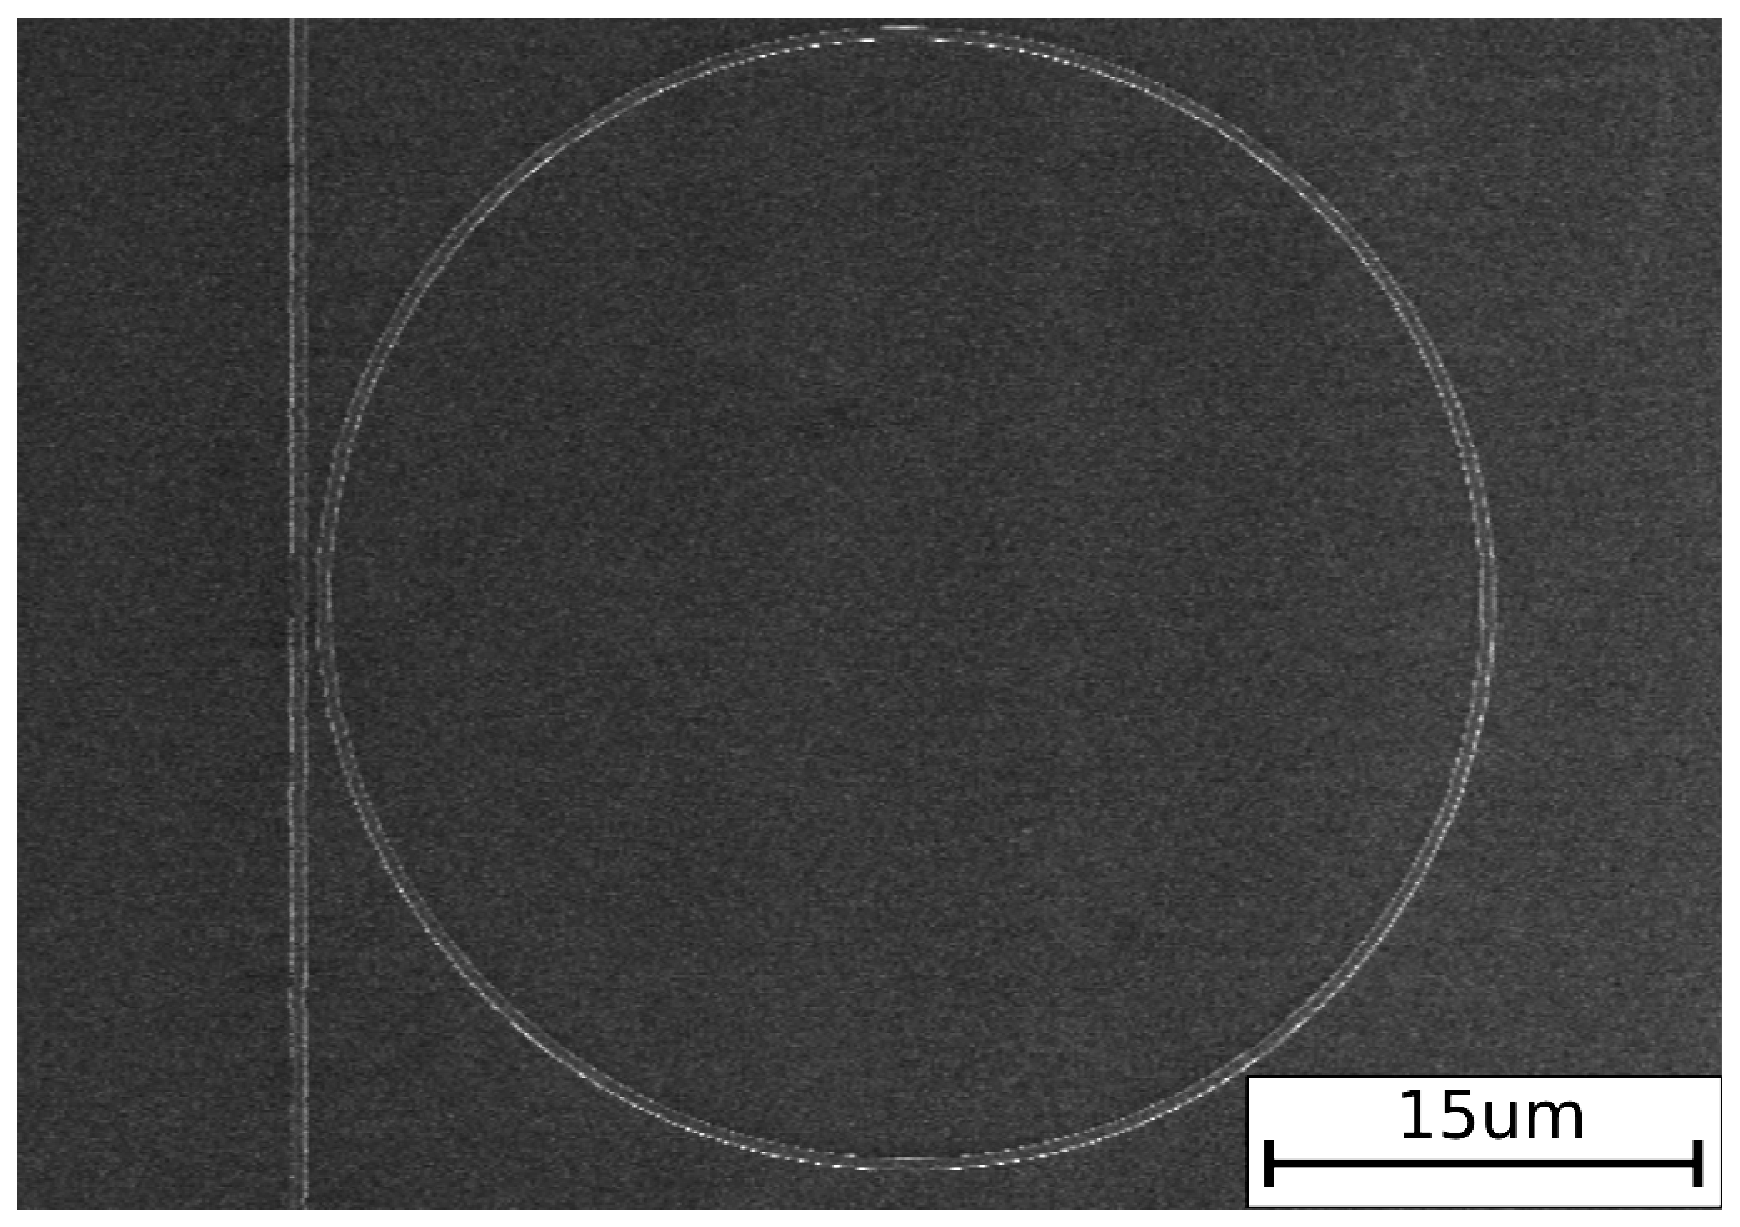
\includegraphics[width=2.5in]{ringTEscale2}
    \caption{SEM micrograph of the 20$\mu$m-radius silicon microring resonator.}
    \label{fig:semRingPaperRings}
\end{figure}


\begin{figure}[htb]
	\centering
	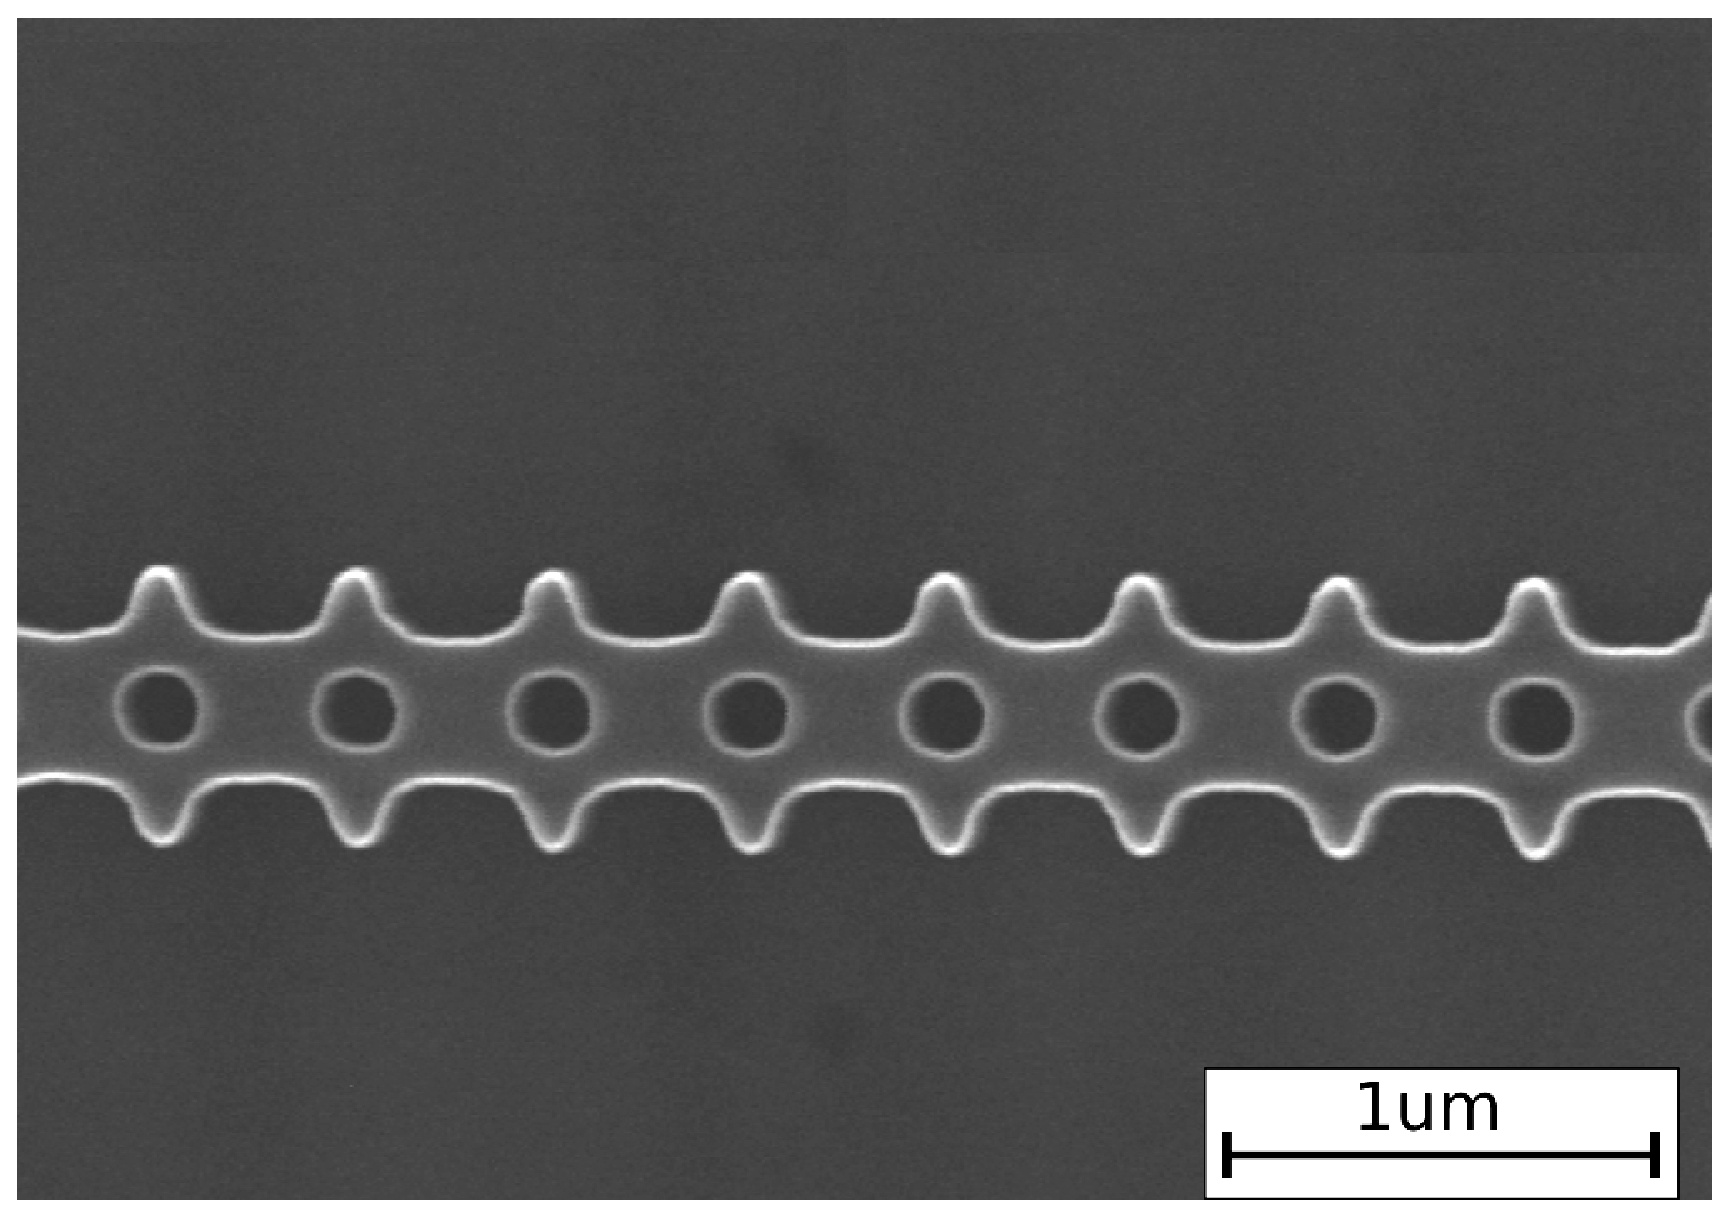
\includegraphics[width=2.5in]{corrTEscale}	
	\caption{SEM micrograph of the corrugated waveguide with a broadband flattened group index profile (from 1560 to 1610~nm), achievable by patterning circular holes onto the wide section of the waveguide as in~\cite{Brimont2010}.}
	\label{fig:sem}
 \end{figure} 


\subsection{Ring resonators parameter extraction}
\label{sec:ringResonators}
Ring resonators are common building blocks, as they can be used as filters, multiplexers, modulators, \emph{etc}~\cite{Bogaerts:12}.
Their spectrum consist of a series of resonances, whose separation is called free spectral range (FSR), which is related to the length and group index of the cavity:

\begin{equation}
	FSR (nm)=\frac{\lambda_{res}^2}{n_gL}
	\label{eq:FSRanillo}
\end{equation} 

where $n_g$ is the group index and $L$ is the round trip length.

The transmission equation of a ring can be easily obtained~\cite{McKinnon2009}:

\begin{equation}
	E_{out}/E_{in}=\frac{t-Ae^{j\beta L}}{1-tAe^{j\beta L}}
\label{eq:transmissionRing}
\end{equation}


where $A$ is the single-pass amplitude transmission and the self ($t$) and cross-coupling ($k$) coefficients of the coupler satisfy $k^2+t^2=1$.

Depending on the relation between the coupling coefficients and the losses ($A=e^{-\frac{\alpha L}{2}}$), a ring resonator can be:

\begin{itemize}
 \item \textbf{Under-coupled ($t>A$):} The coupling is lower than the attenuation through the ring.
 With zero phase at the resonances, each resonance produces a phase fluctuation. 

 \item \textbf{Critically coupled ($t=A$):} The output light coming from the ring and from the input port cancel out, so there is zero transmission at resonance.

 
 \item \textbf{Over-coupled ($t<A$):} The resonance becomes wider (smaller Q-factor) and accumulates an extra $2\pi$ phase shift, because at the output more energy comes from the ring than from the input port, generating an extra phase delay.
 Therefore the phase at the resonance is $\pi$.
\end{itemize}

 

\begin{figure}[htb]
    \centering
    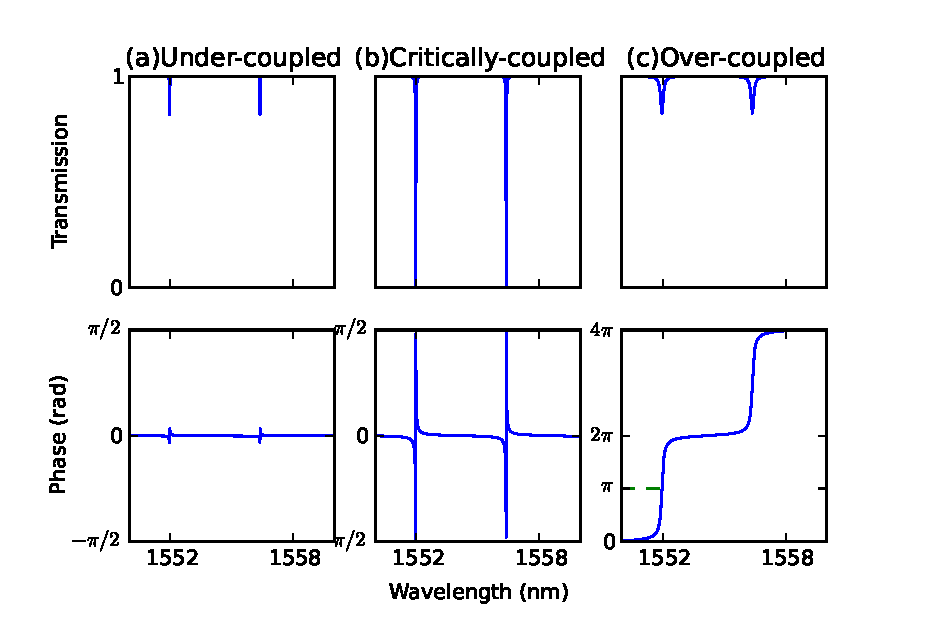
\includegraphics[width=3.5in]{ringCouplingRegimes}
    \caption{Simulated transmission and phase spectra of a ring resonator under different coupling regimes.
    A= 0.99 in all cases, and $t$ is 0.999, 0.99, 0.9 in the left, center and right panels respectively.
    Distinguishing over- from under-coupling regimes requires the phase response.}
    \label{fig:ringDifferentCoupling}
\end{figure}


The procedure for extracting the parameters of a ring resonator usually starts by measuring the FSR to extract the group index, and then focus on a single resonance to extract the loss and the coupling coefficient from a fit.
However, with this method, the under- and over-coupled regimes are indistinguishable, as swapping the loss and coupling parameters generates exactly the same transmission spectrum.
This problem is addressed in Ref.~\cite{McKinnon2009}, where they propose different strategies to disentangle the parameters by looking at many resonances and how they depend on the wavelength.
However, their approach requires some assumptions and measuring a very wide spectral range.
 
With the setup that we propose in this paper, the phase response is also measured, therefore we only need one resonance to determine all the parameters of the ring.
From the phase spectrum, it is straightforward to distinguish the under- from the over-coupled regime as shown in Fig.~\ref{fig:ringDifferentCoupling}.
Fig.~\ref{fig:overcoupled} shows measured and fitted transmission and phase spectra of two different ring resonators using our technique.
The only difference between both rings is the gap between the bus and the ring, which is expected to result in a different coupling coefficient, but similar loss and index.
The phase response allowed us to clearly distinguish the regime, thus the parameters can be easily extracted.
The coupling coefficients obtained (0.350 for the 200~nm gap and 0.217 for the 275~nm gap) follow the expected trend, while the absorption and group index coefficients are very similar.
This, together with the good agreement between experiment and fit, allows us to conclude that the technique successfully provided a complete characterization of the component.


\begin{figure}[htb]
  \centerline{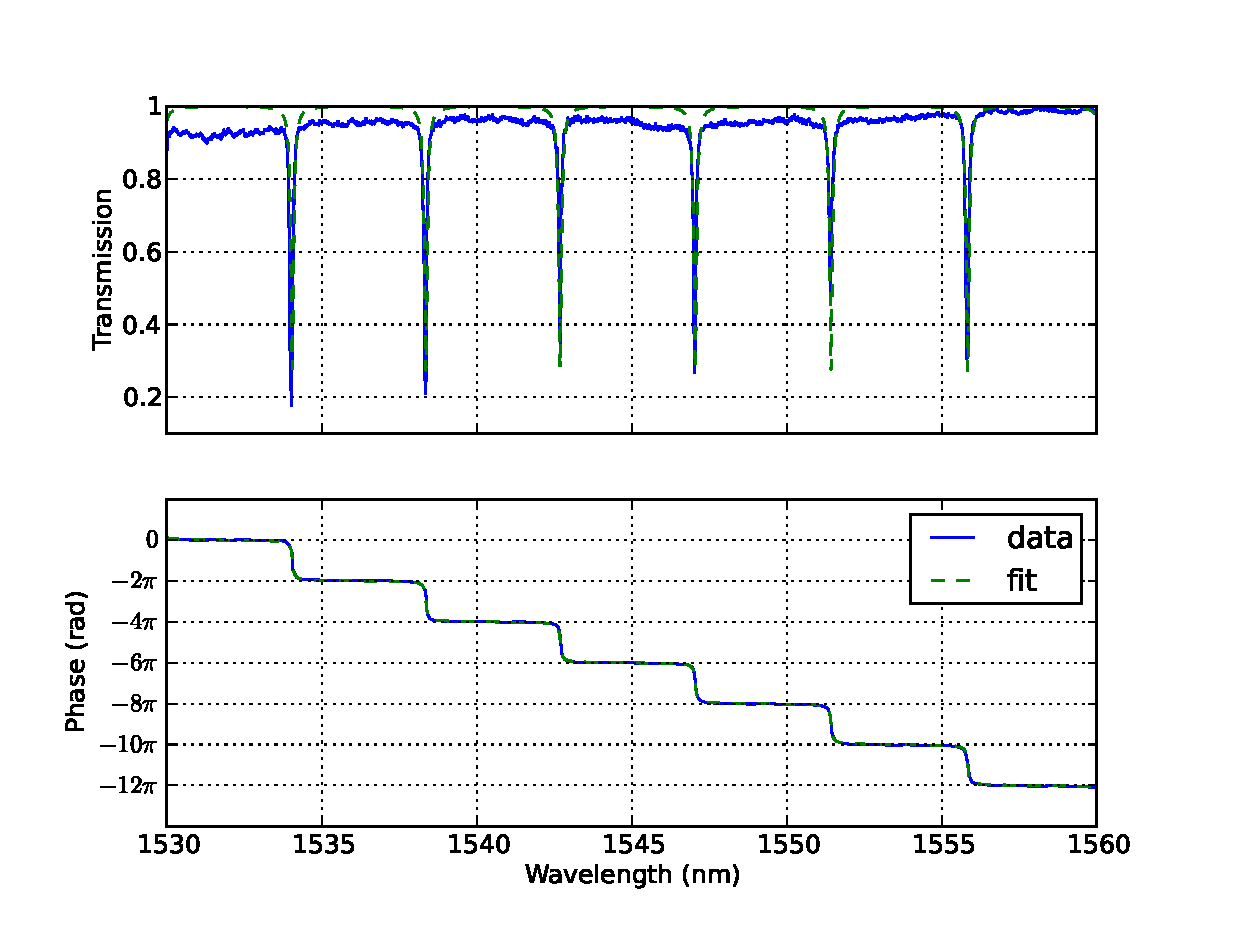
\includegraphics[width=9cm]{r20g200TE_fitPhaseAmp}}
  \centerline{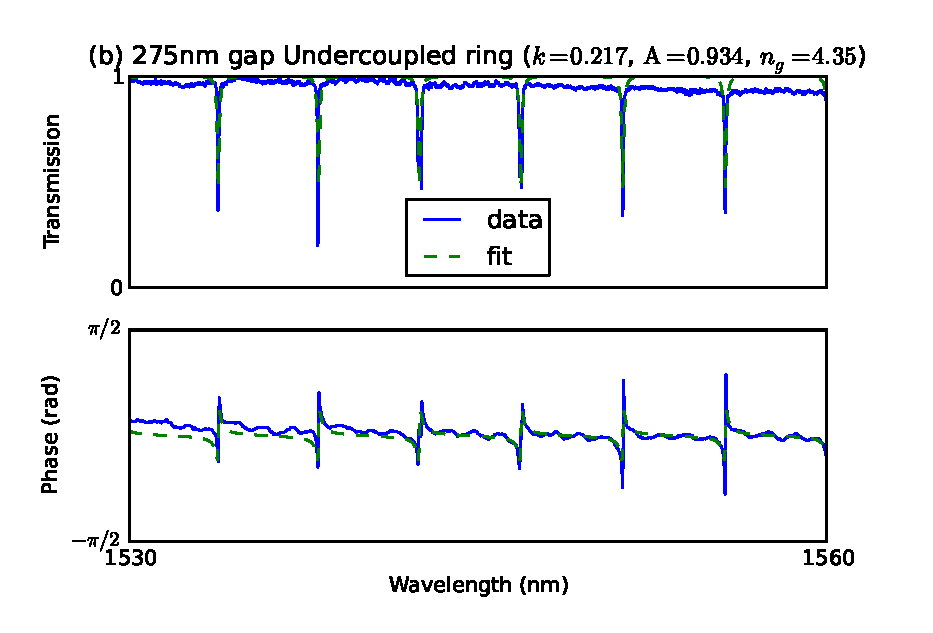
\includegraphics[width=9cm]{r20g275TE_fitPhaseAmp}}
  \caption{Experimental and fitted spectra of two silicon microring resonators. We clearly see that the over-coupled ring (top) accumulates $2\pi$ phase shifts while the under-coupled ring have phase fluctuations in each resonance. }
  \label{fig:overcoupled} % [k = 0.35048909  0.96328564  4.35909895] -25.8545799362 dB/cm 
\end{figure}

\subsection{Group index in slow light corrugated waveguides}
\label{sec:corrWaveguides}
Corrugated waveguides can be employed for dispersion engineering or slow light applications. In these cases, the group index dependence on wavelength is the key parameter. Common techniques to measure it are fringe separation~\cite{shang81,vlasov:05,yao:811,Dulkeith2006} and path balancing~\cite{Cohen:82,Knox:88,Liang:98} of an integrated Mach-Zehnder interferometer. If one branch has the corrugated waveguide and the other one has a reference waveguide with known index, from the wavelength fringe separation ($ \lambda_{min} - \lambda_{max} $) one can obtain the variation of the group index with respect to the photonic wire $ n_{g,ref} $~\cite{vlasov:05}:

%In Fig.~\ref{fig:groupIndex} we show the fringes of an interferometer with a 450~$\mu$m corrugated waveguide in one branch and a reference photonic wire on the other branch.
\begin{figure}[htb]
  \centerline{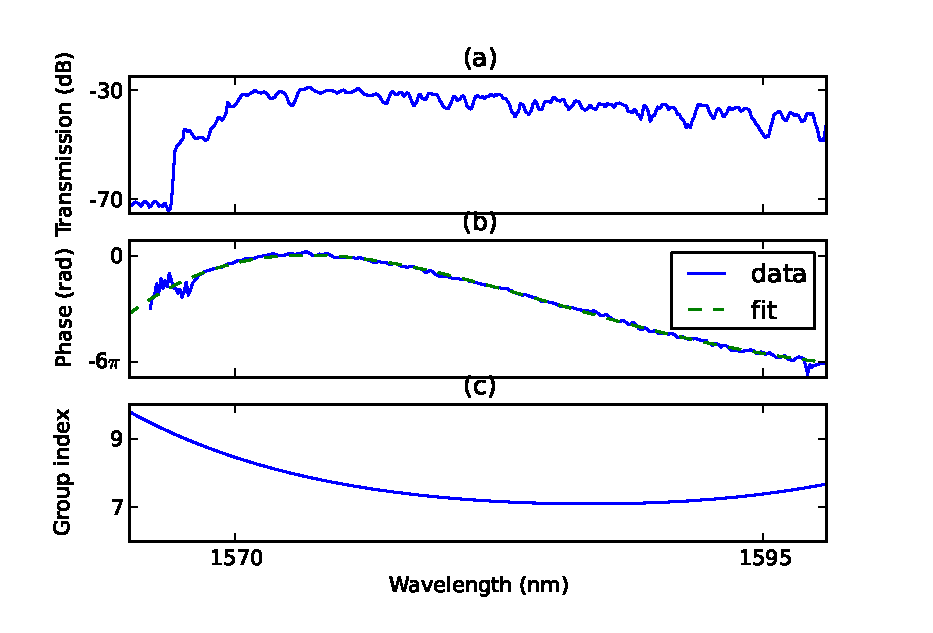
\includegraphics[width=9cm]{corrAmpPhaseResponseGroupIndex}}
%  \caption{(a)~The transmission falls abruptly near the band-gap, where we observe the corrugated group index increase. (b)~Near the band-gap, the phase becomes very noisy, so we fit the phase passband with good transmission. (c)~ Subtracting the phase response of the 450~$\mu$m (b) and a 27 $\mu$m corrugated waveguide we extract the group index of the equivalent 423~$\mu$m corrugated waveguide using eq.~\ref{eq:groupIndexEvolution}.}  
  \caption{450~$\mu$m corrugated waveguide transmission (a) and phase (b). Near the band-gap, the transmission falls abruptly, where we observe the corrugated group index increase (c), that we obtain from the phase response using eq.~\ref{eq:groupIndexEvolution}.}  
 

  \label{fig:corr}
\end{figure}

\begin{equation}
  n_g (\lambda)=\frac{\lambda_{min} \lambda_{max}}{ 2L (\lambda_{min} - \lambda_{max})} + n_{g,ref}
\label{eq:fringes}
\end{equation}

where $n_{g,ref}$ is the group index of the reference branch.

One problem of this technique is that an integrated MZI is necessary; in addition, the group index can only be calculated in discrete points which correspond to the fringe maxima and minima. On the other hand, the technique proposed in this paper can be applied for the characterization of these devices, providing a continuous phase dependence from which we can extract group index with high resolution, only limited by the laser step size (Fig.~\ref{fig:corr}). Moreover it does not require to integrate an interferometer.

Our experimental results show the characterization of a corrugated waveguide using both techniques, the fringe counting and the heterodyne setup shown in Fig.~\ref{fig:dispersionSetup}. The sample is the corrugated waveguide shown in Fig.~\ref{fig:sem}, which was designed to have a flattened slow light band~\cite{Brimont2010}. For the fringe counting technique we used an integrated MZI, one of the branches having a corrugated length of 450~$\mu$m. For the heterodyne characterization, we measured two corrugated waveguides with different lengths, one being 450~$\mu$m and the other one 27~$\mu$m. The subtraction of their responses cancels the coupling elements and system response, only leaving the response of a 423~$\mu$m-long corrugated waveguide.
To balance the interferometer from the short (27~$\mu$m) to the long waveguide (450~$\mu$m), we increased the optical delay line by 11~ps.
This means that an equivalent $L=423~\mu$m-long corrugated waveguide has a group delay $T_g=11$~ps, which corresponds to a group index $n_g(\omega_0)=7.8$ (Eq.~\ref{eq:group_index_pathBalancing}). Then, with the interferometer balanced, we extracted the group index variations around $n_g(\omega_0)$ from the phase evolution slope using this equation:

\begin{equation}
  n_g (\omega)=  n_g(\omega_0) + \frac{c}{L} \frac{d\phi}{d\omega}
 \label{eq:groupIndexEvolution}
\end{equation}

Figure~\ref{fig:groupIndex} shows a comparison between the group index curve obtained with our technique using Eq.~\ref{eq:groupIndexEvolution}, and the points obtained from the fringes of the MZI applying Eq.~\ref{eq:fringes}.
The results agree, but the curve obtained with the heterodyne technique is more immune to the noise, and has the advantage of being continuous rather than scattered.
For these reasons, we consider that the technique proposed in this paper is well suited for the the accurate characterization of this kind of structures.


\begin{figure}[htb]
  \centering
  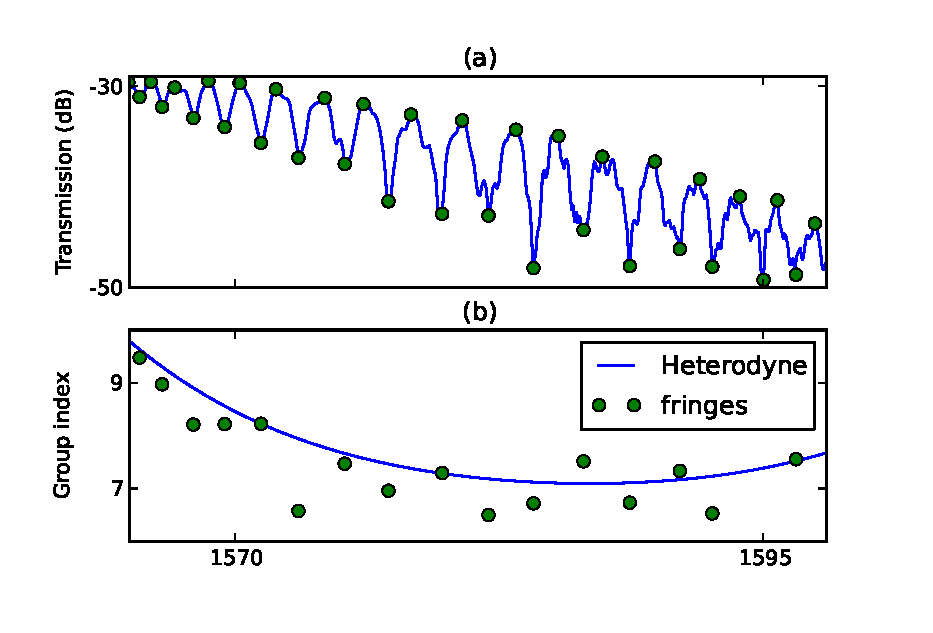
\includegraphics[width=3.5in]{gropIndexComparison_2}
  \caption{(a)~Fringe pattern of an integrated MZI containing the corrugated waveguide on one branch. (b)~Group index results extracted from the fringes (dots) and the heterodyne technique (dashed line).}
  \label{fig:groupIndex}
\end{figure}



\section{Conclusion}
We have shown an experimental technique to characterize the phase response of integrated photonic components.
The technique cancels out phase noise by using a counter-propagating reference beam, avoiding the need of extremely fast tuning rates or cumbersome temperature control schemes.
As examples of application, we characterized a microring resonator and a corrugated waveguide.
From the ring resonator phase response, we clearly distinguished over- from under-coupling regimes, observing an excellent agreement with simulations.
For the corrugated waveguide, we measured the group index profile in the slow-light band with more precision and less noise than using a traditional fringe-spacing method.



\section*{Acknowledgments}
We acknowledge financial support from the Spanish Ministry of Science and Innovation through  SINADEC (TEC2008- 06333), LEOMIS (TEC2012-38540) and PROMETEO/2010/087 NANOFOTONICA contratcs. Universidad Polit\'ecnica de Valencia for PAID2011/1914 and  Joaquin Matres FPI doctoral grant. Transatlantic partnership for Excellence in Engineering (TEE) funded by EU Commission under the Erasmus Mundus Action 2 program is also acknowledged.  We also acknowledge Binbin Guan and Dominique Hainis for fruitful discussions and Jose Angel Ayucar and Javier Garcia-Castello help taking the SEM pictures.


% \bibliographystyle{IEEEtran}
% \bibliography{/home/joaquin/Documents/library}

% Generated by IEEEtran.bst, version: 1.13 (2008/09/30)
\begin{thebibliography}{10}
\providecommand{\url}[1]{#1}
\csname url@samestyle\endcsname
\providecommand{\newblock}{\relax}
\providecommand{\bibinfo}[2]{#2}
\providecommand{\BIBentrySTDinterwordspacing}{\spaceskip=0pt\relax}
\providecommand{\BIBentryALTinterwordstretchfactor}{4}
\providecommand{\BIBentryALTinterwordspacing}{\spaceskip=\fontdimen2\font plus
\BIBentryALTinterwordstretchfactor\fontdimen3\font minus
  \fontdimen4\font\relax}
\providecommand{\BIBforeignlanguage}[2]{{%
\expandafter\ifx\csname l@#1\endcsname\relax
\typeout{** WARNING: IEEEtran.bst: No hyphenation pattern has been}%
\typeout{** loaded for the language `#1'. Using the pattern for}%
\typeout{** the default language instead.}%
\else
\language=\csname l@#1\endcsname
\fi
#2}}
\providecommand{\BIBdecl}{\relax}
\BIBdecl

\bibitem{Vanwiggeren2003}
\BIBentryALTinterwordspacing
G.~D. VanWiggeren, A.~R. Motamedi, and D.~M. Barley, ``{Single-scan
  interferometric component analyzer},'' \emph{Photonics Technology Letters,
  IEEE}, vol.~15, no.~2, pp. 263--265, 2003. [Online]. Available:
  \url{http://ieeexplore.ieee.org/xpls/abs\_all.jsp?arnumber=1174140}
\BIBentrySTDinterwordspacing

\bibitem{Gifford2005}
D.~K. Gifford, B.~J. Soller, M.~S. Wolfe, and M.~E. Froggatt, ``{Optical vector
  network analyzer for single-scan measurements of loss, group delay, and
  polarization mode dispersion},'' \emph{Applied optics}, vol.~44, no.~34, pp.
  7282--7286, 2005.

\bibitem{Dandliker1988}
\BIBentryALTinterwordspacing
R.~D\"{a}ndliker, R.~Thalmann, and D.~Prongu\'{e}, ``{Two-wavelength laser
  interferometry using superheterodyne detection.}'' \emph{Optics letters},
  vol.~13, no.~5, pp. 339--41, May 1988. [Online]. Available:
  \url{http://www.ncbi.nlm.nih.gov/pubmed/19745891}
\BIBentrySTDinterwordspacing

\bibitem{Mas2012}
S.~Mas, J.~Matres, C.~J. Oton, and J.~Mart\'{\i}, ``{Accurate chromatic
  dispersion characterization of photonic integrated circuits},''
  \emph{Photonics Journal, IEEE}, vol.~4, no.~3, pp. 825--831, Jun. 2012.

\bibitem{Brimont2010}
\BIBentryALTinterwordspacing
A.~Brimont, J.~V. Gal\'{a}n, J.~M. Escalante, J.~Mart\'{\i}, and P.~Sanchis,
  ``{Group-index engineering in silicon corrugated waveguides.}'' \emph{Optics
  letters}, vol.~35, no.~16, pp. 2708--10, Aug. 2010. [Online]. Available:
  \url{http://www.ncbi.nlm.nih.gov/pubmed/20717431}
\BIBentrySTDinterwordspacing

\bibitem{Bogaerts:12}
\BIBentryALTinterwordspacing
W.~Bogaerts, P.~{De Heyn}, T.~{Van Vaerenbergh}, K.~{De Vos}, S.~{Kumar
  Selvaraja}, T.~Claes, P.~Dumon, P.~Bienstman, D.~{Van Thourhout}, and
  R.~Baets, ``{Silicon microring resonators},'' \emph{Laser \& Photonics
  Reviews}, vol.~6, no.~1, pp. 47--73, 2012. [Online]. Available:
  \url{http://dx.doi.org/10.1002/lpor.201100017}
\BIBentrySTDinterwordspacing

\bibitem{McKinnon2009}
\BIBentryALTinterwordspacing
W.~R. McKinnon, D.~X. Xu, C.~Storey, E.~Post, a.~Densmore, a.~Del\^{a}ge,
  P.~Waldron, J.~H. Schmid, and S.~Janz, ``{Extracting coupling and loss
  coefficients from a ring resonator.}'' \emph{Optics express}, vol.~17,
  no.~21, pp. 18\,971--82, Oct. 2009. [Online]. Available:
  \url{http://www.ncbi.nlm.nih.gov/pubmed/20372631}
\BIBentrySTDinterwordspacing

\bibitem{shang81}
H.-T. Shang, ``{Chromatic dispersion measurement by white-light interferometry
  on metre-length single-mode optical fibres},'' \emph{Electronics Letters},
  vol.~17, no.~17, pp. 603--605, 1981.

\bibitem{vlasov:05}
Y.~A. Vlasov, M.~O'Boyle, H.~F. Hamann, and S.~J. McNab, ``{Active control of
  slow light on a chip with photonic crystal waveguides},'' \emph{Nature}, vol.
  438, no. 7064, pp. 65--69, 2005.

\bibitem{yao:811}
\BIBentryALTinterwordspacing
X.~S. Yao and J.~Feinberg, ``{Simple in-line method to measure the dispersion
  of an optical system},'' \emph{Applied Physics Letters}, vol.~62, no.~8, pp.
  811--813, 1993. [Online]. Available:
  \url{http://link.aip.org/link/?APL/62/811/1}
\BIBentrySTDinterwordspacing

\bibitem{Dulkeith2006}
\BIBentryALTinterwordspacing
E.~Dulkeith, F.~Xia, L.~Schares, W.~M.~J. Green, L.~Sekaric, and Y.~A. Vlasov,
  ``{Group index and group velocity dispersion in silicon-on-insulator photonic
  wires.}'' \emph{Optics express}, vol.~14, no.~13, p. 6372, Jun. 2006.
  [Online]. Available:
  \url{http://www.ncbi.nlm.nih.gov/pubmed/19516814}
\BIBentrySTDinterwordspacing

\bibitem{Cohen:82}
L.~G. Cohen and J.~Stone, ``{Interferometric measurements of minimum dispersion
  spectra in short lengths of single-mode fibre},'' \emph{Electronics Letters},
  vol.~18, no.~13, pp. 564--566, 1982.

\bibitem{Knox:88}
\BIBentryALTinterwordspacing
W.~H. Knox, N.~M. Pearson, K.~D. Li, and C.~A. Hirlimann, ``{Interferometric
  measurements of femtosecond group delay in optical components},'' \emph{Opt.
  Lett.}, vol.~13, no.~7, pp. 574--576, Jul. 1988. [Online]. Available:
  \url{http://ol.osa.org/abstract.cfm?URI=ol-13-7-574}
\BIBentrySTDinterwordspacing

\bibitem{Liang:98}
\BIBentryALTinterwordspacing
Y.~Liang and C.~P. Grover, ``{Modified white-light Mach-Zehnder interferometer
  for direct group-delay measurements},'' \emph{Appl. Opt.}, vol.~37, no.~19,
  pp. 4105--4111, Jul. 1998. [Online]. Available:
  \url{http://ao.osa.org/abstract.cfm?URI=ao-37-19-4105}
\BIBentrySTDinterwordspacing

\end{thebibliography}

\extraSpace

% \usepackage[labelformat=empty]{caption}
% \usepackage[labelformat=empty]{caption}
% \usepackage{caption}


\begin{wrapfigure}{l}{1in}
\includegraphics[width=1in]{joaquin}
% joaquin.eps: 0x0 pixel, 300dpi, 0.00x0.00 cm, bb=-0 -0 781 781
\end{wrapfigure}

\textbf{Joaquin Matres} received his Engineering (2009) and M.Sc. (2010) degree in Telecommunications from the Universidad Politecnica de Valencia. He is currently in a Research Stay at the University of California, Davis and finishing his PhD in the Valencia Nanophotonics Technology Center. He is involved in studying the nonlinear properties of silicon based nanophotonic waveguides, with the goal of making CMOS-compatible all-optical devices, including switches and logic gates.
\extraSpace

\begin{wrapfigure}{l}{1in}
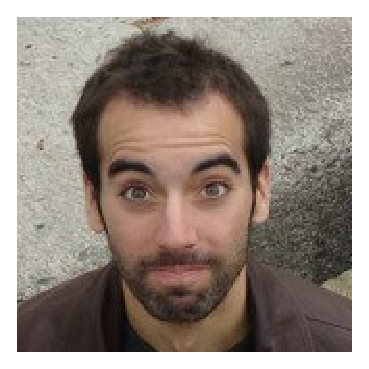
\includegraphics[width=1in]{guillem}
% joaquin.eps: 0x0 pixel, 300dpi, 0.00x0.00 cm, bb=-0 -0 781 781
\end{wrapfigure}

\textbf{Guillem Ballesteros} received his Physics degree from Universidad de Valencia in 2010 and continued his education in the Universidad Politecnica de Valencia while employed as a junior researcher at the Valencia Nanophotonics Technology Center. Here he obtained his M.Sc. degree in Telecommunications (2012). Currently, he is working towards his PhD at Eidgen\"{o}ssische Technische Hochschule Z\"{u}rich (ETHZ), working on developing and calibrating simulation tools to study the early stages of tumorigenesis.
\extraSpace

\begin{wrapfigure}{l}{1in}
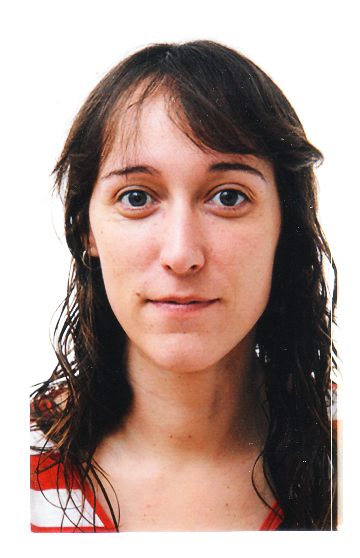
\includegraphics[width=1in]{sara}
% joaquin.eps: 0x0 pixel, 300dpi, 0.00x0.00 cm, bb=-0 -0 781 781
\end{wrapfigure}

\textbf{Sara Mas} received his Engineering degree in Telecommunications in 2009 from the Universidad de Cantabria and M.Sc. degree in 2010 from the Universidad Politecnica de Valencia. She is currently working towards his PhD in the Valencia Nanophotonics Technology Center. Her research interests include chromatic dispersion and nonlinear effects in silicon integrated waveguides and optical frequency combs using microresonators.
\extraSpace



\begin{wrapfigure}{l}{1in}
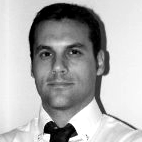
\includegraphics[width=1in]{antoine}
% joaquin.eps: 0x0 pixel, 300dpi, 0.00x0.00 cm, bb=-0 -0 781 781
\end{wrapfigure}
\textbf{Antoine Brimont} was born in Valence, France, in 1982. He received the Engineering Master's Degree in Materials Science and Nanotechnology from the Institut National des Sciences Appliquees (INSA) de Rennes, France, as well as the M.Sc in Physics in collaboration with the University of Rennes, in 2005. He also received the Ph.D. in Telecommunications Engineering from the Polytechnic University of Valencia, Spain, in 2011. He is currently working as a senior research engineer at the Valencia Nanophotonics Technology Center, Spain. His research interests include integrated silicon photonics and specifically high speed silicon modulators. He has authored or co-authored over 40 papers in peer-reviewed international journals and international conferences.
\extraSpace

\begin{wrapfigure}{l}{1in}
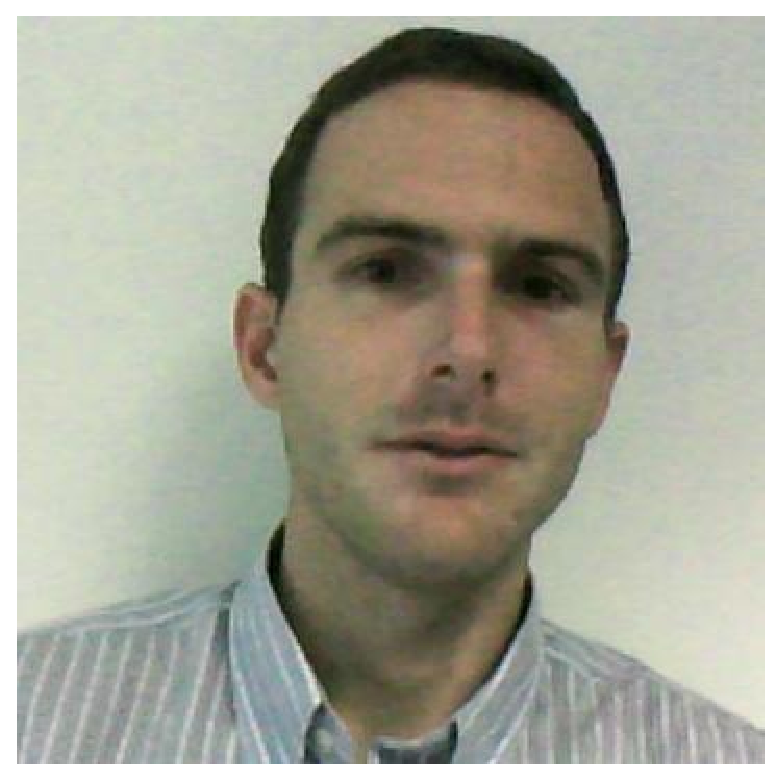
\includegraphics[width=1in]{pablo}
% joaquin.eps: 0x0 pixel, 300dpi, 0.00x0.00 cm, bb=-0 -0 781 781
\end{wrapfigure}

\textbf{Pablo Sanchis} received the Ingeniero de Telecomunicacion degree (M.Sc.) and the Doctor Ingeniero de Telecomunicacion degree (Ph.D.) from the Universidad Politecnica de Valencia, Valencia, Spain, in 2001 and 2005 respectively. He is full-time associate professor at the Universidad Politecnica de Valencia and senior researcher member of the Valencia Nanophotonics Technology Centre where he currently leads a research group in optical modulators. His research interests include modelling, design and fabrication issues in integrated optics, especially in the field of silicon photonics. He has been involved in several national research projects and European research projects (FP5-OBANET, FP6-PHOLOGIC, FP6-ePIXnet, FP7-HELIOS). He has authored more than 48 papers in peer-reviewed international journals and more than 85 papers in international conferences and he holds several patents.
\extraSpace

\begin{wrapfigure}{l}{1in}
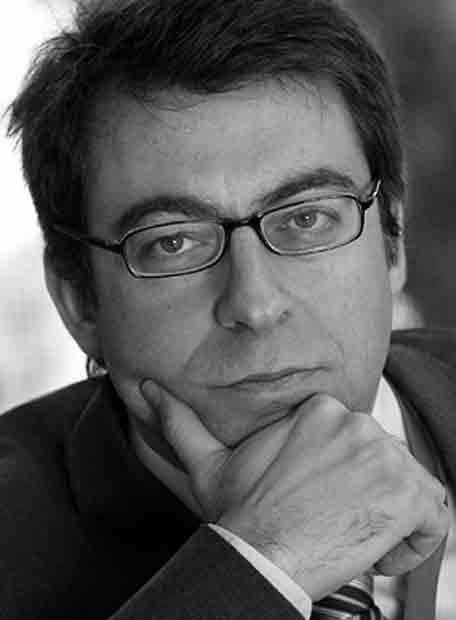
\includegraphics[width=1in]{javier}
% joaquin.eps: 0x0 pixel, 300dpi, 0.00x0.00 cm, bb=-0 -0 781 781
\end{wrapfigure}
\textbf{Javier Marti} received the Ingeniero de Telecomunicacion degree from the Universitat Politecnica de Catalunya, Catalunya, Spain, in 1991, and the Doctor Ingeniero de Telecomunicacion degree (Ph.D.) from the Universidad Politecnica de Valencia, (UPVLC) Spain, in 1994. Since 2000 he holds a Full-Professor position at the Telecommunication Engineering Faculty at UPVLC. In 2003 he was appointed Director of the Valencia Nanophotonics Technology Centre (NTC), that includes a silicon photonics facility with several research activities in areas as metamaterials and plasmonics, photonic integrated devices, microwave photonics and high-speed optical networks. In 2005 he founded DAS PHOTONICS, a spin-off company of NTC, aimed to develop proprietary photonics technology for high end markets such as  defence, avionics and space. Prof. Marti is currently President of DAS PHOTONICS.
He has co-authored over 20 patents and more thanr 300 papers in refereed international technical journals in the fields of opto-microwave systems and technologies, Silicon photonics circuits and high-speed optical communications.
The research of Javier Marti has always being motivated towards industry and commercial applications and has pioneered industrial research developments with leading world-class companies and organisations like European Research Agency, European Defense Agency and European Southern Observatory. He has led many national and international research projects focused on photonic technology and system, and has acteds the co-ordinator of many industrial consortia in the European Framework Programs. He is a founder and member of the Board of Stakeholders of the European Technology Platform Photonics 21. He has served as member of the Programme Committee of OFC, ECOC, MWP, Group IV Photonics and many other international conferences.
\extraSpace

\begin{wrapfigure}{l}{1in}
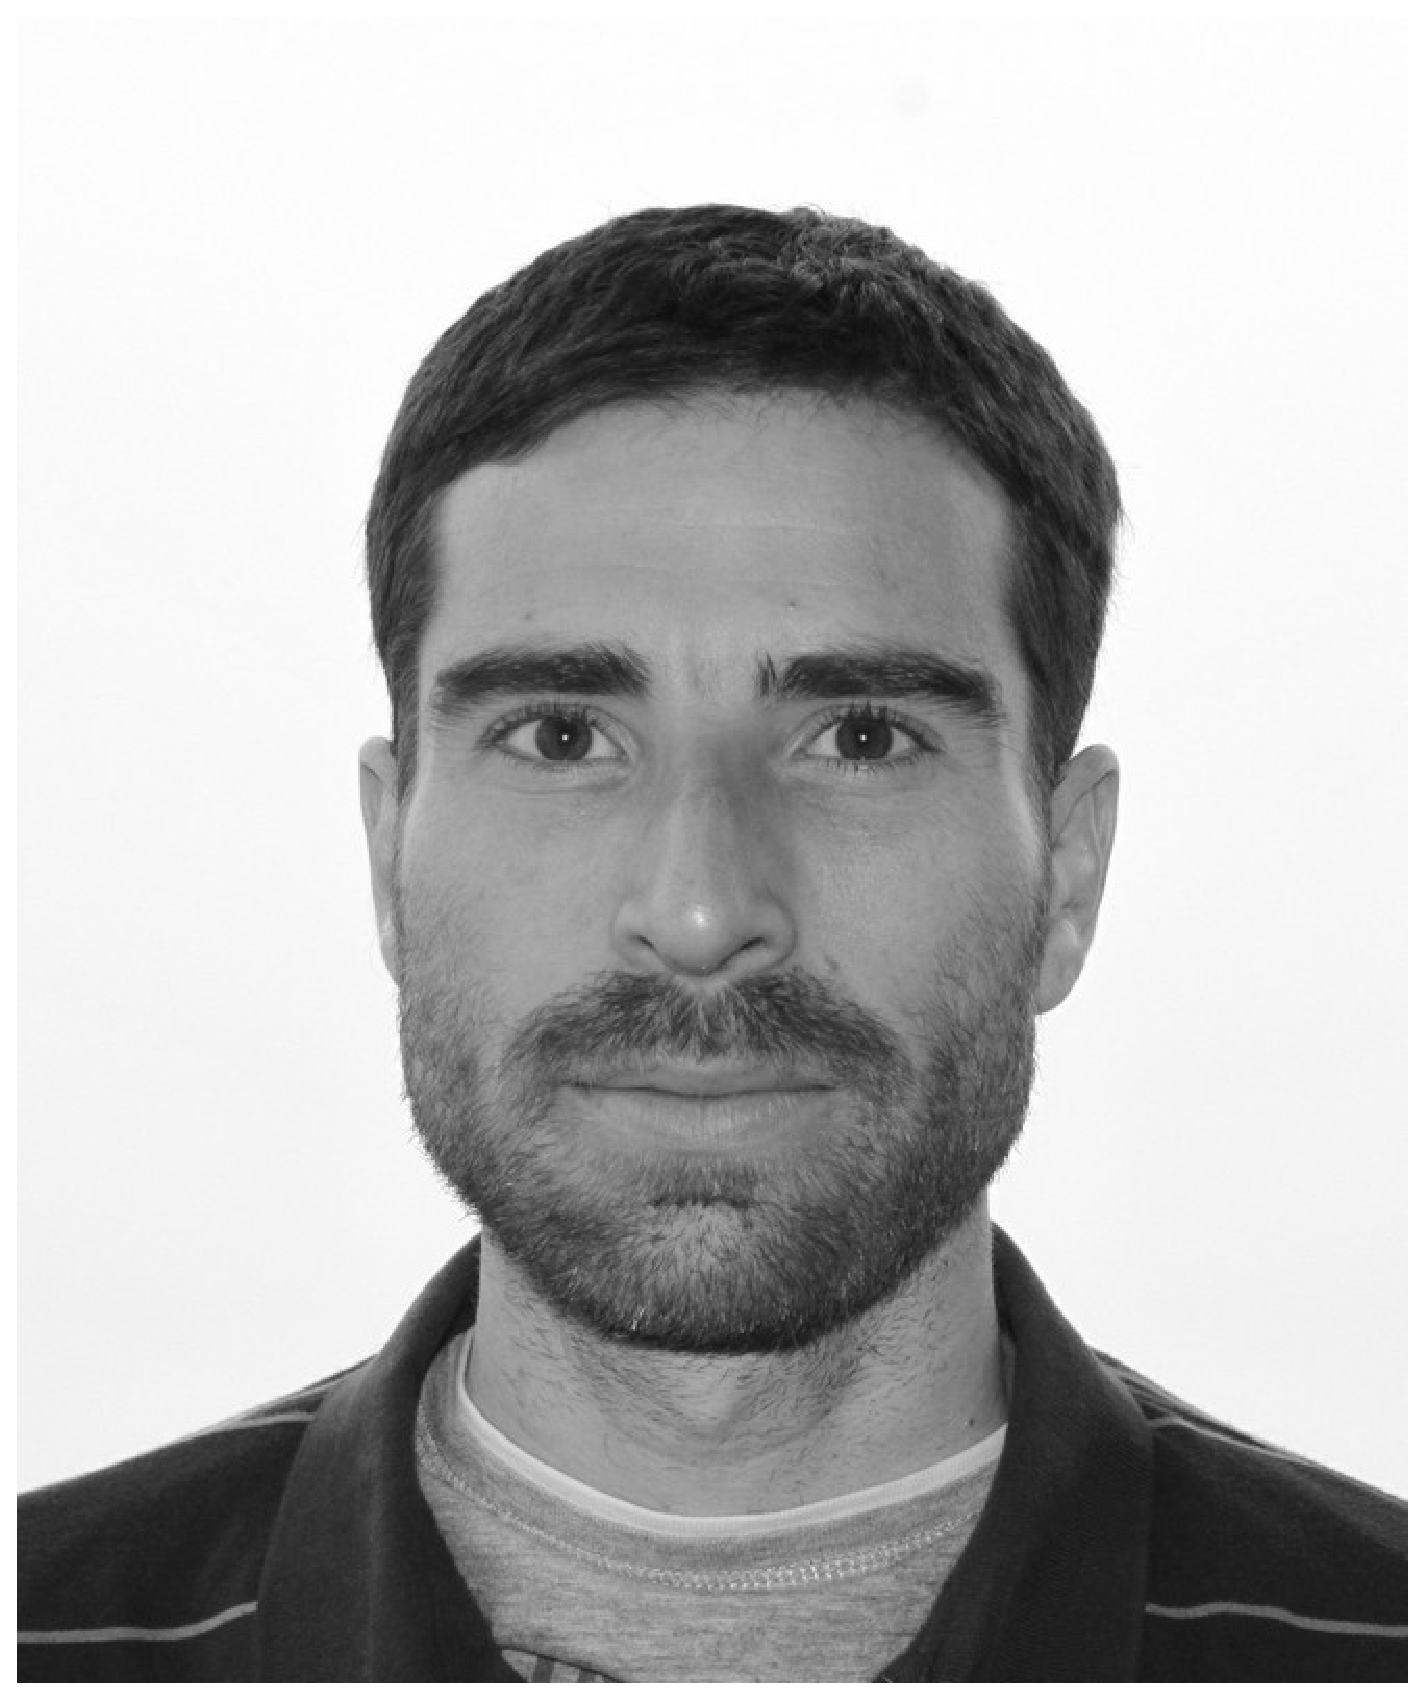
\includegraphics[width=1in]{claudio}
\end{wrapfigure}
\textbf{Claudio Oton} obtained his PhD in 2005 in University of La Laguna (Spain), and he has spent 4 years in University of Southampton (UK) as a post-doc Research Fellow, 3 years in Universidad Politecnica de Valencia (Spain) as a Senior Research Fellow, and in 2012 he joined Scuola Superiore Sant'Anna (Italy) as an Assistant Professor. He has published more than 50 peer-reviewed research papers and has participated in numerous research projects, funded by the EU and the British, Spanish and Italian national programs. His current fields of expertise are silicon photonics and optical fiber sensors.


\end{document}

